% Basic setup
\documentclass[12pt,a4paper]{article} % Defines the document type as an article with 12pt font size on A4 paper.

% Importing packages
\usepackage[english]{babel} % Sets the document language to English, adjusting hyphenation and language-specific typographic rules.
\usepackage[lmargin=2.5cm,rmargin=2.5cm,tmargin=2.5cm,bmargin=2.5cm]{geometry} % Sets custom page margins: left/right 2.5cm, top 2.5cm, bottom 2.5cm.

% Loading packages
\usepackage{amsmath}
\usepackage{hyperref}    % Enables hyperlinks for references, URLs, and citations.
\usepackage{xcolor}      % Provides tools for defining and using colors.
\usepackage{graphicx}    % Allows inclusion of images and graphics.
\usepackage{caption}     % Customizes captions for figures and tables.
\usepackage{subcaption}  % Supports subfigures and subcaptions within figures.
\usepackage{minted}      % Enables syntax highlighting for code listings.
\usepackage[T1]{fontenc} % Ensures proper font encoding, important for correct character rendering. Don't touch this.
\usepackage{lmodern}     % Sets the font to something more modern and easy to read.
\usepackage{setspace}    % Provides control over line spacing.
\usepackage{csquotes}    % Improves handling of quotations.
\usepackage{setspace}    % Used to set line spacing
\usepackage{longtable,booktabs,array} % Packages for advanced table formatting.
\usepackage{wasysym}
\usepackage[
  backend=biber,
  style=apa,  
]{biblatex}  % Manages citations and bibliography with APA style.

\setstretch{1.5} % Sets line spacing

\definecolor{LightGray}{gray}{0.9}  % Defines a custom color 'LightGray' with 90% gray, used for the code block background.
\hypersetup{                        % Configures hyperlink colors and behavior.
  colorlinks=true,                  % Enable colored links instead of boxes.
  linkcolor={blue},                 % Sets link color to blue.
  filecolor={maroon},               % Sets file link color to maroon.
  citecolor={blue},                 % Sets citation link color to blue.
  urlcolor={blue}}                  % Sets URL link color to blue.

\addbibresource{assets/bib-template.bib} % Adds the bibliography file.

\title{Place Holder page titre}        % Sets the document title.
\makeatletter
\providecommand{\subtitle}[1]{%     % Custom command to add a subtitle.
  \apptocmd{\@title}{\par {\large #1 \par}}{}{}
}

\makeatother
\subtitle{Va être remplacée par celle sur Teams}  % Sets the document subtitle.
\author{Charles Bouthillier Paul Charvet William Hamilton Samuel Roy}% Sets the author's name.
\date{2025-12-12}                   % Sets the document date.

% \renewcommand{\familydefault}{\sfdefault} % Changes the default font to one without serifs

% From this point, the preamble ends and the actual content of the document starts.
\begin{document}
\pagenumbering{gobble} % Stops counting the pages from this point until changed again.
\maketitle
%\begin{abstract}
%This is the LaTeX template (\textbf{Version 1.1}) from the DH Lab of the University of Basel. It is suitable for Seminar Papers and Master's / PhD theses, but can be adapted to fit a variety of use cases. It was created by Stefan Freitag and is derived from the Quarto template, which is also available from the DH Lab.

%The abstract of your paper / thesis goes right here. It will appear on the cover sheet (very first page) of the PDF, together with the title, subtitle, author name and date.

%If you do not want your document to have an abstract, you can also simple delete the 'abstract' part (or comment it out) with all its content and the final document will be created without it.
%\end{abstract}
\begin{center}
    \vfill
    \begin{figure}[H] 
          \includegraphics[width=.8\linewidth]{./assets/Université_Laval_logo_et_texte.svg.png}
    \end{figure}
        \setcounter{figure}{0}
        
    Université Laval\\
    Facutlé de science génie\\
    Québec
\end{center}
\newpage
\renewcommand*\contentsname{Table des matières} % This controls the title of your table of contents.
{
\hypersetup{linkcolor=}
\setcounter{tocdepth}{5} % Sets the maximum sublevel to be displayed within the table of contents.

\tableofcontents
}
\newpage
\pagenumbering{arabic}\setstretch{1.5} % Overwrites the previous command, pages are counted as normal from this point.


\section{Vue CAD 3D explosée}
    \begin{figure}[H] 
	    \includegraphics[width=1.1\linewidth]{./assets/Explose.png}
    \end{figure}

\section{captures d'écran des enveloppes d'impression}

\subsection{Volumes Préférentiels X-Y}
    \subsubsection{Lot \#1}    
    \begin{figure}[H] 
	    \includegraphics[width=1.1\linewidth]{./assets/XY_pref1.pdf}
    \end{figure}
    \subsubsection{Lot \#2}
    \begin{figure}[H] 
	    \includegraphics[width=1.1\linewidth]{./assets/XY_pref2.pdf}
    \end{figure}

\subsection{Volumes Préférentiels Z} 
    \subsubsection{Lot \#3}    
    \begin{figure}[H] 
	    \includegraphics[width=1.1\linewidth]{./assets/Z_pref1.pdf}
    \end{figure}
    \subsubsection{Lot \#4}
    \begin{figure}[H] 
	    \includegraphics[width=1.1\linewidth]{./assets/Z_pref2.pdf}
    \end{figure}

\section{Croquis à main levé}

    \subsection{Concept \#1: Charles Bouthillier}
    \begin{figure}[H] 
	    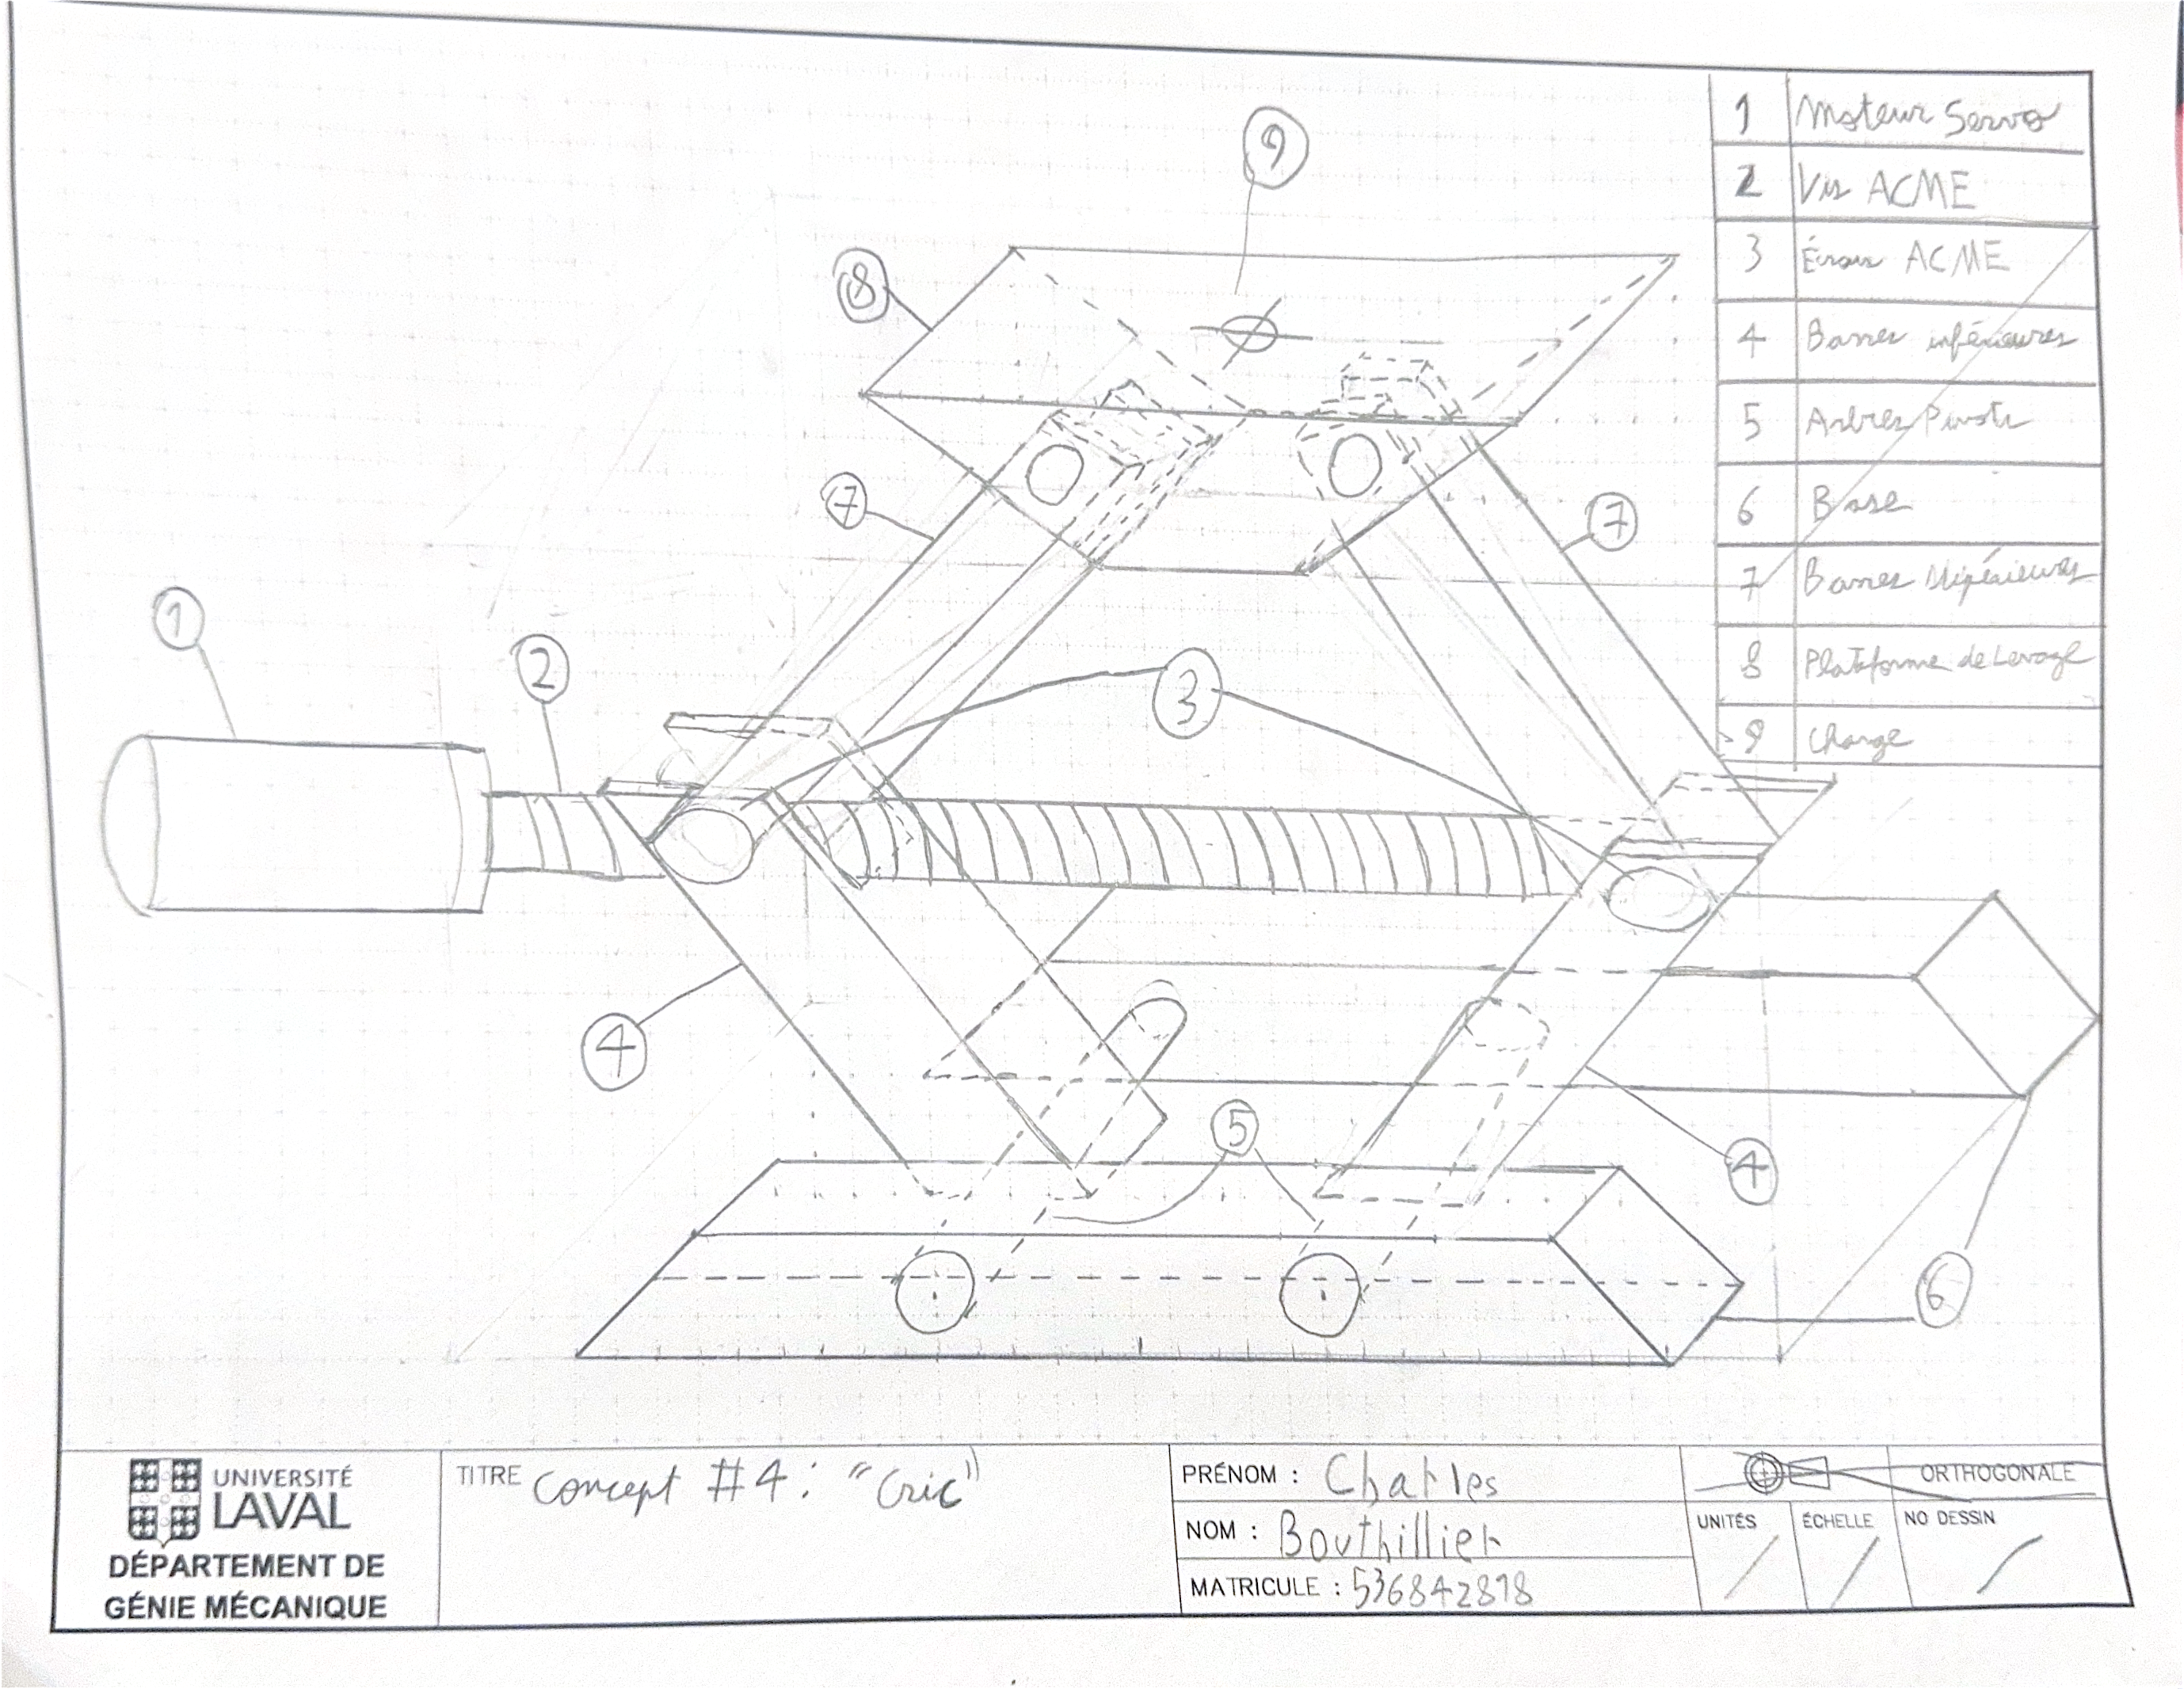
\includegraphics[width=1.1\linewidth]{./assets/Croquis_CB.pdf}
    \end{figure}
    \begin{par}
	    Explication du concept: Cette solution est inspiré d'un "cric" permettant de soulever des voitures. Le moteur (\#1) fait tourner une vis ACME (\#2). Deux écrous (\#3) sont bloqués en rotation sur la vis, lorsque le moteur tourne, ils seront naturellement pousser vers le centre de la vis, entrainant avec eux les pivots centraux des barres (\#4 et \#7). Lorsque les pivots centraux se rapprochent, les systèmes de barres se dressent, ce qui a pour efffet d'élever la plateforme (\#8), et par extension, la charge (\#9) qui y est posée.
    \end{par}
    \begin{figure}[H] 
	    \includegraphics[width=0.45\linewidth]{./assets/Signatures/Signature_CB.png}
    \end{figure}

    \subsection{Concept \#2: Samuel Roy}
    \begin{figure}[H] 
	    \includegraphics[width=1.1\linewidth]{./assets/Croquis_SR.pdf}
    \end{figure}
    \begin{par}
	    Explication du concept:
	    Voir image ci-dessus
    \end{par}
    \begin{figure}[H] 
	    \includegraphics[width=0.45\linewidth]{./assets/Signatures/Signature_SR.png}
    \end{figure}

    \subsection{Concept \#3: Paul Charvet}
    \begin{figure}[H] 
	    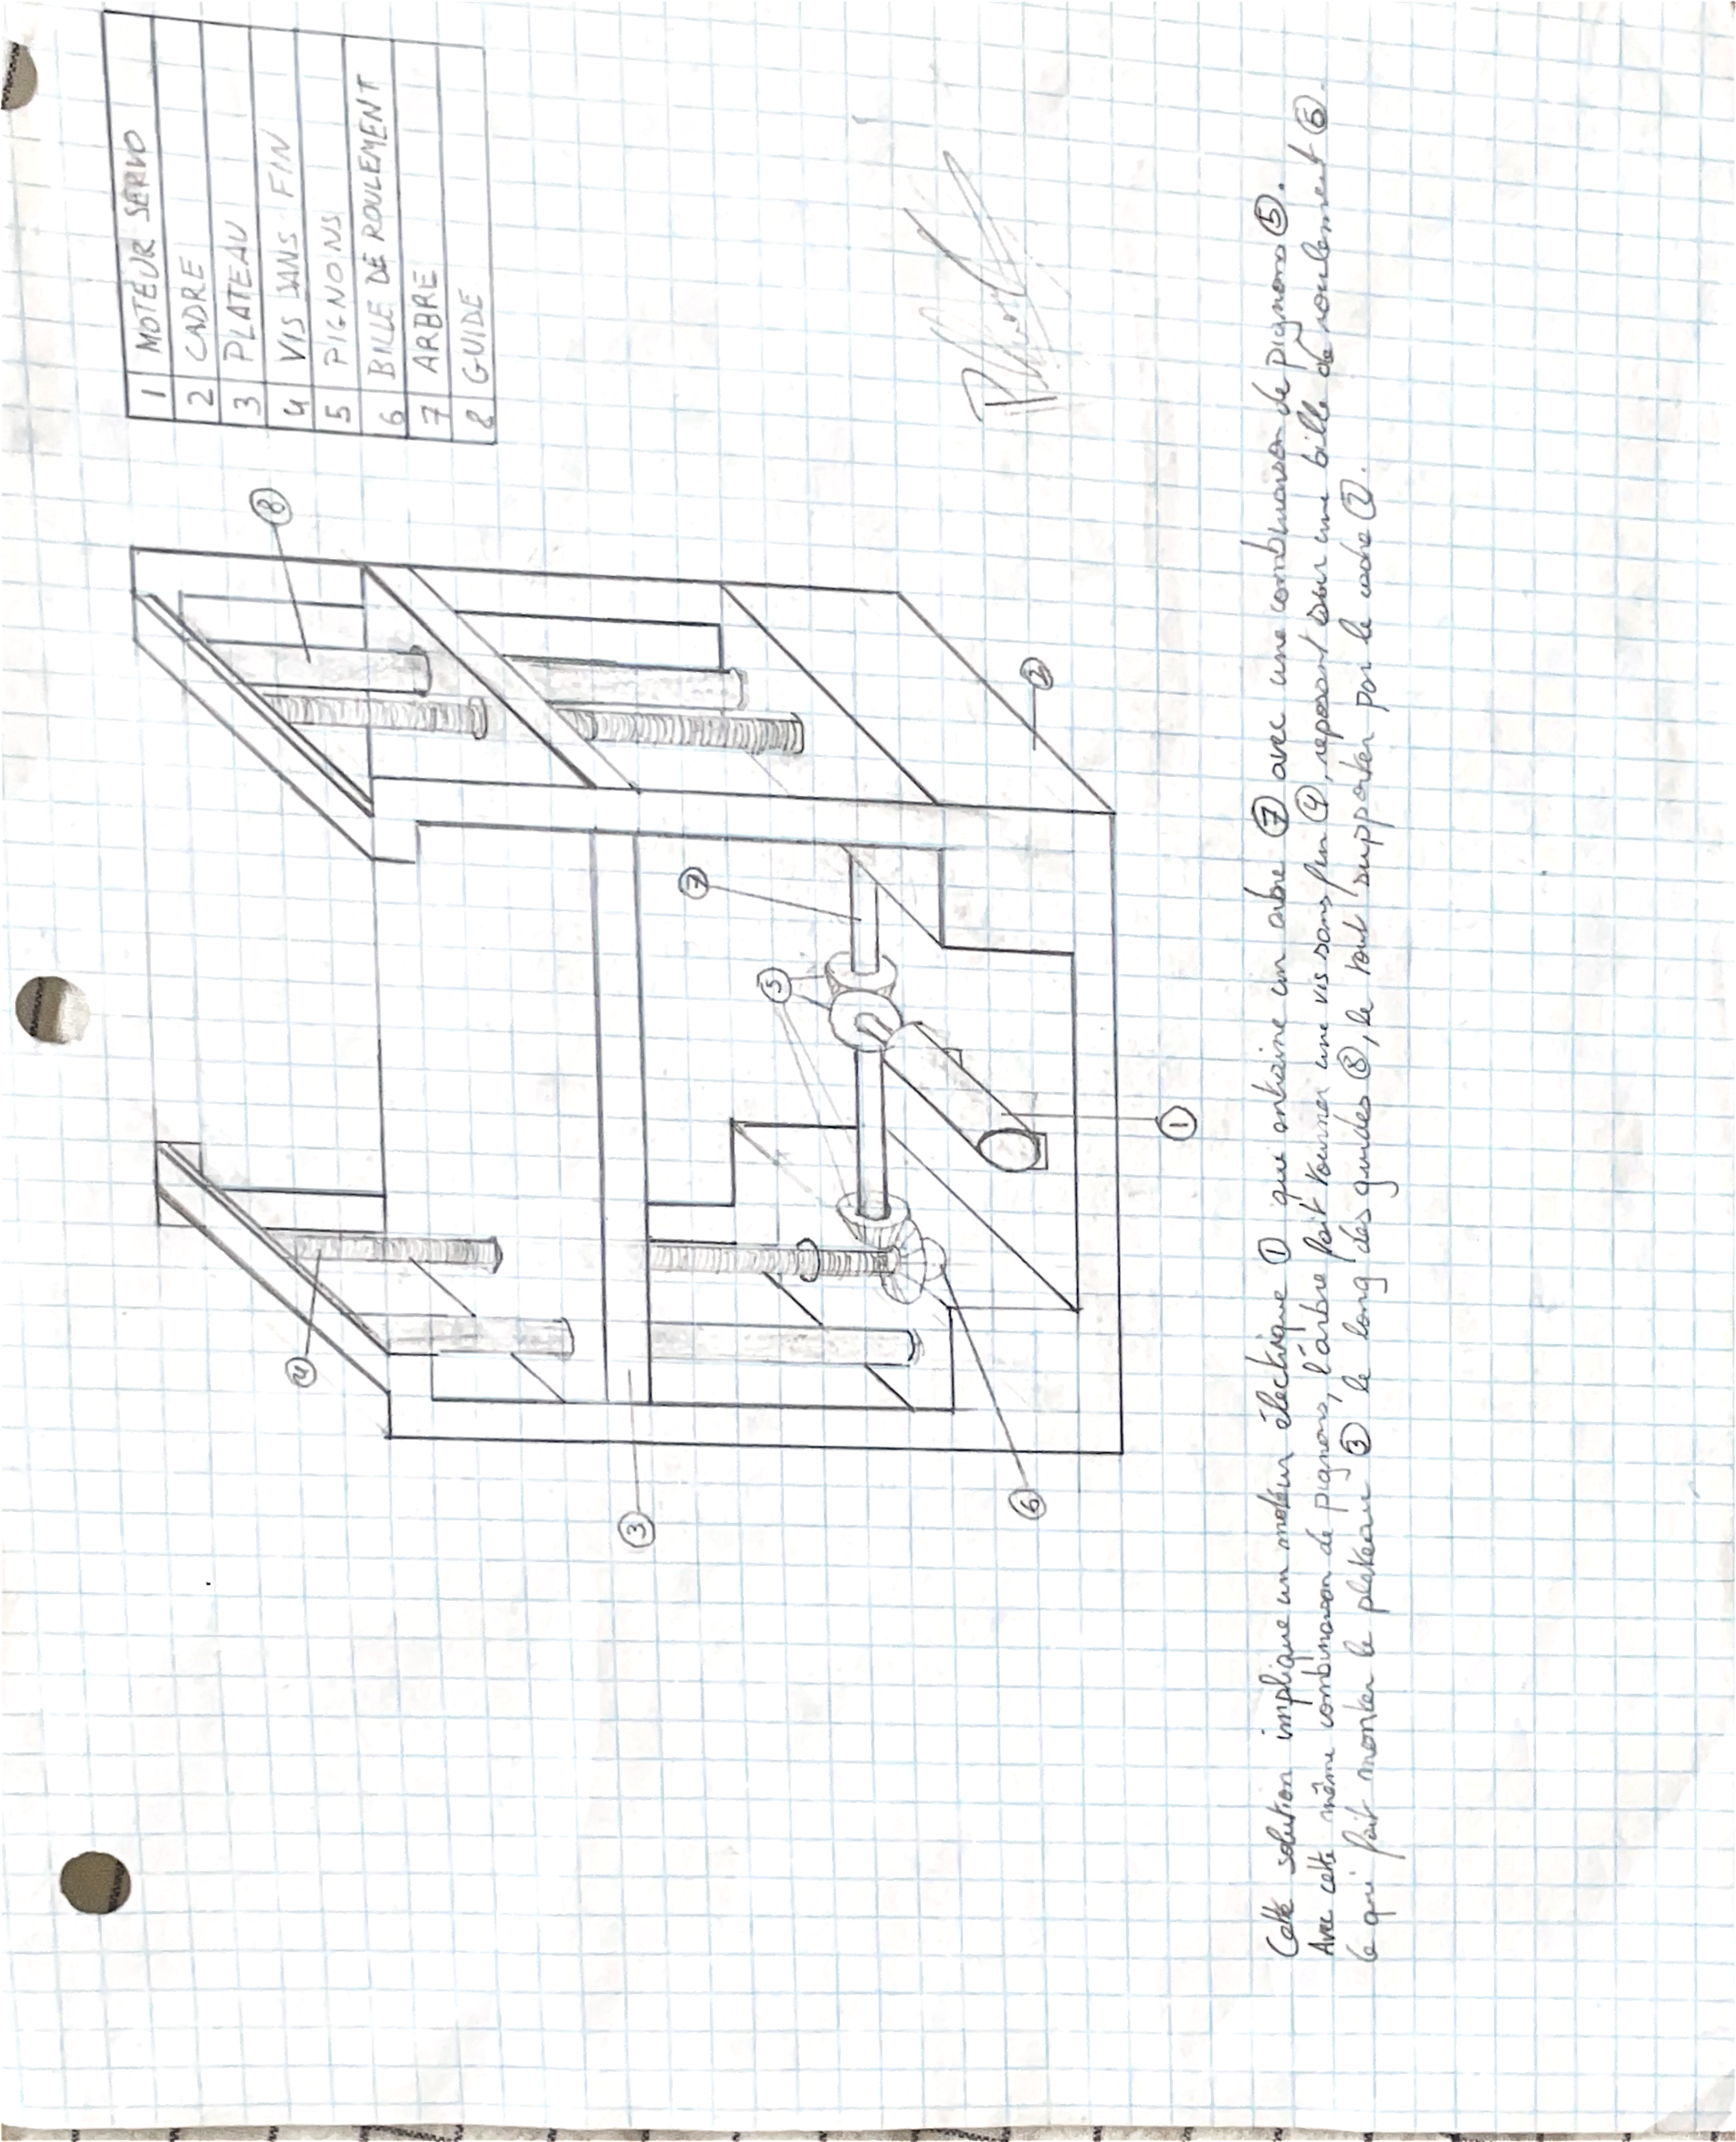
\includegraphics[width=1.1\linewidth]{./assets/Croquis_PC.pdf}
    \end{figure}
    \begin{par}
	    Explication du concept: Cette solution implique un moteur électrique (\#1) qui entraine un arbre (\#7) avec une combinaison de pignons (\#5). À l'aide de cette dernière, l'arbre fait tourner une vis sans fin (\#4) reposant sur une bille de roulement (\#6), ce qui fait monter le plateau (\#3) le long des guides (\#8), le tout supporter par le cadre (\#2). 
    \end{par}
    \begin{figure}[H] 
	    \includegraphics[width=0.30\linewidth]{./assets/Signatures/Signature_PC.png}
    \end{figure}

    \subsection{Concept \#4: William Hamilton}
    \begin{figure}[H] 
	    \includegraphics[width=1.1\linewidth]{./assets/croquis_WH.jpg}
    \end{figure}
    \begin{par}
	    Explication du concept: Le moteur électrique (\#1) entraine l'arbre (\#2). Cet arbre entraîne la roue dentée (\#3). La roue dentée contient des filets intérieurs pour permettre à la vis sans fin (\#4) d'être dévissée et de faire monter la plateforme (\#5). Le mécanisme est dons le bâti (\#6).
    \end{par}
    \begin{figure}[H] 
	    \includegraphics[width=0.45\linewidth]{./assets/Signatures/Signature_WH.png}
    \end{figure}

    \subsection{Grille de sélection}
    \begin{figure}[H] 
	    \includegraphics[width=1.1\linewidth]{./assets/Grille.png}
    \end{figure}
    \subsection{Justification des cotes}
    \begin{par}
Pour le concept \#1, nous avons décidé d’attribuer la note de 60/100 au critère de propension à soulever une charge importante, en raison des contraintes susceptibles d’être appliquées aux pièces 5, dites « arbres pivots », lesquelles pourraient avoir des difficultés à les supporter.
Concernant la variabilité du niveau de charge pouvant être soulevée en fonction de la géométrie, nous estimons que, lorsque le système se rapproche de sa hauteur maximale, la répartition des contraintes est amenée à évoluer. Bien que nous n’ayons pas réalisé d’analyse approfondie, nous avons choisi d’attribuer une note de 80/100.
La complexité du mécanisme ainsi que le nombre de pièces ont été jugés raisonnables ; c’est pourquoi une note de 80/100 a été retenue pour ce critère.
Enfin, le niveau d’incertitude a également obtenu cette note, dans la mesure où il s’agit d’un concept déjà connu et couramment utilisé.
    \end{par}
\vspace{\baselineskip}
    \begin{par}
Pour le concept \#2, nous avons estimé que la capacité à soulever une charge importante serait limitée et que le couple requis atteindrait rapidement une valeur susceptible de bloquer le moteur. De plus, l’engrenage 5 risquerait de frotter contre le fond du boîtier. Pour ces raisons, nous avons attribué une note de 65/100.
Ensuite, bien que nous n’ayons réalisé ni calculs ni analyses détaillées, nous avons supposé que la hauteur du système n’influencerait pas sa capacité à soulever différentes charges. Ainsi, une note de 100/100 a été attribuée pour ce critère.
En ce qui concerne la complexité et le nombre de pièces, ce concept est de loin le plus simple ; la note de 95/100 lui a donc été accordée. Les cinq points retirés s’expliquent par la conception des pièces 2 et 5, respectivement la « worm gear » et la « wheel gear », jugée plus exigeante.
Enfin, une note de 70/100 a été attribuée en raison des incertitudes liées au système de transmission de puissance ainsi que du risque de flambage de la pièce 4, la « structure de guidage ».
    \end{par}
\vspace{\baselineskip}
    \begin{par}
Le concept \#3 a été jugé capable de soulever une charge importante, avec une note de 80/100, en raison de la présence de deux pièces 4, des « vis sans fin ». Toutefois, un travail d’optimisation des rapports de transmission aurait été nécessaire afin de garantir une meilleure capacité de reprise de charge.
Nous estimons que ce concept est parfaitement capable de supporter la charge indépendamment de la hauteur de la pièce 3, le « plateau », grâce aux pièces 8, les « guides ». C’est pourquoi la note de 100/100 a été attribuée pour ce critère.
En revanche, ce concept présente une complexité élevée, avec un grand nombre de pièces en mouvement, ce qui justifie la note de 30/100.
Enfin, concernant le niveau d’incertitude et de risque associé à ce concept, celui-ci a été jugé relativement faible. En effet, le système est très stable grâce aux guides et à la pièce 2, le « cadre », et une part importante des efforts est reprise par des pièces métalliques (4 et 6).
    \end{par}
\vspace{\baselineskip}
    \begin{par}
Pour le concept \#4, nous estimons que, bien qu’il soit très résistant, il présente un problème similaire à celui du concept 2, à savoir une variation de rapport de transmission insuffisante, susceptible d’entraîner le blocage du moteur. Une note de 70/100 a donc été attribuée.
En ce qui concerne la capacité de levage en fonction de la hauteur, nous avons jugé que l’impact serait limité ; c’est pourquoi une note de 90/100 a été accordée.
Nous avons également estimé que ce concept était peu complexe, car il comporte un nombre relativement réduit de pièces.
Enfin, nous avons considéré que la géométrie conique conférait une robustesse accrue au système, réduisant ainsi le risque de rupture.
    \end{par}
\section{Calculs}

\subsection{Calcul de faisabilité (\#1)}
	\subsubsection{DCL des composantes dans le chemin de force}	
\begin{enumerate}
\renewcommand{\labelenumi}{\alph{enumi})}
  \begin{minipage}{\linewidth}
  \item
  Moteur

  \medskip
  \includegraphics[width=1\linewidth]{./assets/DCL/Moteur.png}
  \end{minipage}
  \begin{minipage}{\linewidth}
  \item
  Vis sans fin

  \medskip
  \includegraphics[width=1\linewidth]{./assets/DCL/Worm.png}
  \end{minipage}
  \begin{minipage}{\linewidth}
  \item
  Roue dentée

  \medskip
  \includegraphics[width=1\linewidth]{./assets/DCL/Gear1.png}
  \end{minipage}
  \begin{minipage}{\linewidth}
  \item
  arbre au centre de la roue dentée

  \medskip
  \includegraphics[width=0.75\linewidth]{./assets/DCL/Shaft.png}
  \end{minipage}
  \begin{minipage}{\linewidth}
  \item
  Pignon 

  \medskip
  \includegraphics[width=1\linewidth]{./assets/DCL/Gear2.png}
  \end{minipage}
  \begin{minipage}{\linewidth}
  \item
  Écrou ACME

  \medskip
  \includegraphics[width=1\linewidth]{./assets/DCL/ACME_nut.png}
  \end{minipage}
  \begin{minipage}{\linewidth}
  \item
  Vis ACME

  \medskip
  \includegraphics[width=0.7\linewidth]{./assets/DCL/ACME_screw.png}
  \end{minipage}
\end{enumerate}
	\subsubsection{couple pour soulever 295,5kg}
\begin{center}
	\begin{tabular}{|c c c|}
		\hline
		Paramètre & symbole & valeur de base\\
		\hline
		masse à soulever & $M_{charge}$ & 295,5 [kg]\\
	constante de gravité & g & 9,81 [ $ms^{-2}}$ ]\\
	pas de la vis ACME & P & 0,00254 [m]\\
	Diamètre primitif vis ACME & $\diameter_s$ & 0,011285 [m]\\
	lead angle vis ACME& $\lambda_v$ & N/A [$\circ$]\\
	angle d'hélice vis ACME& $\psi_v$ & 4,098 [$\circ$]\\
	coeff. friction vis-écrou & $\mu$ & 0,5 [-]\\
	coeff. friction nylon-nylon & f & 0,25 [-]\\
	efficacité & $\varepsilon$ & N/A [-]\\
	Torque pour soulever la charge & $T_c$ & N/A [Nm]\\
	rayon primitif du pinion & $R_g$ & 0,01915 [m]\\
	Perte de torque en friction au pinion & $T_f$ & N/A [Nm]\\
	Torque au pinion & $T_a$ & N/A [Nm]\\
	nombre de dents du pinion & $Z_a$ & 29 [-]\\
	nombre de dents de la roue dentée & $Z_b$ & 53 [-]\\
	efficacité engrenage hélicoïdal & $\eta$ & 0,98 [-]\\
	angle de pression & $\phi_n$ & 20 [$\circ$]\\
	angle d'hélice vis sans fin& $\psi_w$ & 3,5 [$\circ$]\\	
	efficacité engrenage vis sans fin & $e_w$ & N/A [-]\\
	nombre de filets vis sans fin & $Z_w$ & 2 [-]\\
	Couple du moteur & $C_{mot}$ & N/A [Nm]\\

		\hline
	\end{tabular}
\end{center}
\begin{enumerate}
  \renewcommand{\labelenumi}{\alph{enumi})}

  \item Torque pour soulever la charge
\[ \lambda = atan(\frac{P}{\pi*\diameter_s}) = 4,098 \]

\[ \varepsilon = \frac{tan(\psi)}{tan(\psi+atan(\mu))} = 0,1208 \]

\[ T_c = \frac{M_{charge}*g*P}{2\pi*\varepsilon} = 9,7 \]
  \item Transmission de torque entre la roue dentée et le pinion
	  \[ T_f = \frac{1}{2}f*M_{charge}*g*R_g=6,94 \]
\[ T_a = T_f+ T_c = 16,64  \]
\[ T_b = \eta*\frac{Z_b}{Z_a}*T_a = 29,21 \]
  \item Transmission de torque entre la roue dentée et la vis sans fin
\[ e_w = \frac{cos(\phi_n) - f*tan(\psi)}{cos(\phi_n) + f*cot(\psi)} = 0,18388 \]
\[ C_{mot} = T_{worm} = \frac{T_b*Z_w}{e_w*Z_b} = 6 > 1,2 Nm \]
Couple trop grand, il faut diminuer la charge sur le système
\end{enumerate}
	\subsubsection{couple pour soulever une charge optimale (34/75 kg/lbs})
\begin{center}
	\begin{tabular}{|c c c|}
		\hline
		Paramètre & symbole & valeur de base\\
		\hline
		masse à soulever & $M_{charge}$ & 34 [kg]\\
		\hline
	\end{tabular}
\end{center}

\begin{enumerate}
  \renewcommand{\labelenumi}{\alph{enumi})}

  \item Torque pour soulever la charge
	  \[ T_c = \frac{M_{charge}*g*P}{2\pi*\varepsilon} = 1,114 \]
  \item Transmission de torque entre la roue dentée et le pinion
	  \[ T_f = \frac{1}{2}f*M_{charge}*g*R_g=0,797 \]
\[ T_a = T_f+ T_c = 1,911  \]
\[ T_b = \eta*\frac{Z_b}{Z_a}*T_a = 3,354 \]
  \item Transmission de torque entre la roue dentée et la vis sans fin
\[ C_{mot} = T_{worm} = \frac{T_b*Z_w}{e_w*Z_b} = 0,689 < 1,2 Nm \]
\end{enumerate}
	\subsubsection{masse pour un couple moteur unitaire}
\begin{center}
	\begin{tabular}{|c c c|}
		\hline
		Paramètre & symbole & valeur de base\\
		\hline
		couple moteur & $C_{mot}$ & 1 [Nm]\\
		masse à soulever & $M_{charge}$ & N\A [kg]\\
		\hline
	\end{tabular}
\end{center}
\begin{enumerate}
  \renewcommand{\labelenumi}{\alph{enumi})}
  \item Transmission de torque entre le moteur et la roue dentée
\[ T_{w} = C_{mot} = 1 \]
\[ T_{b} = \frac{T_w*e_w*Z_b}{Z_w}= 4,8728 \]
  \item Transmission de torque entre la roue dentée et le pinion
\[ T_a = \frac{1}{\eta}*\frac{Z_a}{Z_b}*T_b = 2,72 \]
\[ T_c = T_a - T_f\]
  \item Torque pour soulever la charge
	  \[ M_{charge} = \frac{(T_a-T_f)*2\pi*\varepsilon}{g*P} \]

	  \[ M_{charge} = \frac{(T_a-\frac{1}{2}f*M_{charge}*g*R_g)*2\pi*\varepsilon}{g*P} \]

	  \[ M_{charge} = \frac{2*T_a*\pi*\varepsilon}{g*(P+f*R_g*\pi*\varepsilon)} = 48,30 kg \]

\end{enumerate}

	\subsubsection{temps de montée}
\begin{center}
	\begin{tabular}{|c c c|}
		\hline
		Paramètre & symbole & valeur de base\\
		\hline
		vitesse du moteur & $N_{mot}$ & 233 [rpm]\\
		nombre de filets de la vis sans fin & Z_w & 2 [-]\\
		nombre de dents de la roue dentée & Z_b & 53 [-]\\
		vitesse de la roue dentée & \omega_b & N/A [rpm]\\
		nombre de dents du pinion & Z_a & 29 [-]\\
		vitesse dy pinion & \omega_a & N/A [-]\\
		distance de levage & d & 0,04 [m]\\
		Pas de la vis ACME & P & 0,00254 [m]\\
		temps de levage & t_{montée} & N/A [s]\\
		\hline
	\end{tabular}
\end{center}
\[ \omega_b = \frac{N_{mot}*Z_w}{Z_b} = 8,79 \]

\[ \omega_a = \frac{\omega_{b}*Z_b}{Z_a} = 16,069 [RPM] = 0,268 [Hz] \]

\[ t_{montée} = \frac{d}{\omega_{a}*P} = 58,8 < 60 \]


\begin{center}
	\begin{tabular}{|c c c|}
		\hline
		Paramètre & symbole & valeur de base\\
		\hline
		couple moteur & $C_{mot\_boost}$ & 2,2 [Nm]\\
		masse à soulever & $M_{surcharge}$ & N/A [kg]\\
		\hline
	\end{tabular}
\end{center}

\subsubsection{Évaluer la surcharge}
\begin{center}
	\begin{tabular}{|c c c|}
		\hline
		Paramètre & symbole & valeur de base\\
		\hline
		couple moteur & $C_{mot\_boost}$ & 2,2 [Nm]\\
		masse à soulever & $M_{surcharge}$ & N/A [kg]\\
		\hline
	\end{tabular}
\end{center}
\begin{enumerate}
  \renewcommand{\labelenumi}{\alph{enumi})}
  \item Transmission de torque entre le moteur et la roue dentée
\[ T_{w} = C_{mot\_boost} = 2,2 \]
\[ T_{b} = \frac{T_w*e_w*Z_b}{Z_w}= 10,72 \]
  \item Transmission de torque entre la roue dentée et le pinion
\[ T_a = \frac{1}{\eta}*\frac{Z_a}{Z_b}*T_b = 5,984 \]
\[ T_c = T_a - T_f\]
  \item Torque pour soulever la charge
	  \[ M_{surcharge} = \frac{(T_a-T_f)*2\pi*\varepsilon}{g*P} \]

	  \[ M_{surcharge} = \frac{(T_a-\frac{1}{2}f*M_{surcharge}*g*R_g)*2\pi*\varepsilon}{g*P} \]

	  \[ M_{surcharge} = \frac{2*T_a*\pi*\varepsilon}{g*(P+f*R_g*\pi*\varepsilon)} = 106,26 kg \]

\end{enumerate}
\begin{table}[h]
\caption{Spécifications du système}
\begin{center}
	\begin{tabular}{|c c c|}
		\hline
		Paramètre & symbole & valeur de base\\
		\hline
		couple moteur d'opération & $C_{mot}$ & 0,689 [Nm]\\
		masse admissible & $M_{charge}$ & 34 [kg]\\
		vitesse du moteur & $N_{mot}$ & 233 [rpm]\\
		temps de levage & $t_{montée}$ & 58,8 [s]\\
		limite de surcharge & $M_{surcharge}$ & 106,26 [kg]\\
		\hline
	\end{tabular}
\end{center}
\end{table}

\subsection{Calcul \#2: flexion des dents de la roue dentée (pièce \#1)}
\subsubsection{explication des contraintes physiques}
Les dents de la roue dentée subissent une force dans le plan de le roue aux niveaux des engrenages avec le pignon et la vis sans fin. Ces forces sont causées par la transmission de puissance de la vis sans fin au pinion par le bias de la roue dentée. Elles sont donc égales puisque proportionelle au couple passant par la roue, ainsi qu'à la distance centre-point d'application, qui est la même.Ces forces tendent à faire fléchir les dents, d'où l'intérêt du calcul d'un bris flexural. 
\subsubsection{DCL}
  \includegraphics[width=1\linewidth]{./assets/DCL/dent_wg.png}
\subsubsection{données techniques du calculs}
\begin{center}
	\begin{tabular}{|c c c|}
		\hline
		Paramètre & symbole & valeur de base\\
		\hline
		largeur de la dent & t & VAL [m]\\
		hauteur de la dent & l & VAL [m]\\
		profondeur de contact & F & VAL [m]\\
		Couple nominal à la roue dentée & $T_{b}$ & 3,354 [Nm]\\
		diamètre primitif de la roue dentée & $d_{wg}$ & 0,070 [m]\\
		force tangentielle sur la roue dentée & $W_{twg}$ & N/A [N]\\
		\hline
	\end{tabular}
\end{center}
\subsubsection{question technique et description du calcul}
Question : Quel chargement entrainera la rupture des dents de la roue dentée en flexion?\\
Calcul : Utiliser l'équation de Lewis appliquée aux engrenages pour trouver la contrainte de flexion présente à la base des dents en opération normale et trouver le facteur de sécurité en fonction de la limite flexurale du Nylon. Ensuite, poser la contrainte de flexion à la base des dents comme étant la limite flexurale, et vérifier la charge correspondante pour conclure sur le bris des dents lors de l'essai de surcharge.
\subsubsection{cas en opération normale}
\begin{enumerate}
  \renewcommand{\labelenumi}{\alph{enumi})}
  \item force tangentielle au cercle primitif de la roue dentée
	  \[ W_{twg} = \frac{2*T_{b}}{d_wg} = 95,83 \]
  \item contrainte de flexion appliquée sur la dent
	  \[ \sigma_{b} = \frac{MC}{I} = \frac{6W_{twg}l}{Ft^2} = 17,952 [MPa] \]
  \item facteur de sécurité en opération normale

	  \[ F.S = \frac{S_{e}}{\sigma_b}=2,34 > 1,25 \]
Les dents de la roue dentée ne devraient pas fléchir en opération normale

\subsubsection{cas en surcharge}
\begin{enumerate}
  \renewcommand{\labelenumi}{\alph{enumi})}
  \item force tangentielle au cercle primitif de la roue dentée
	  \[ W_{twg} = \frac{Se*F*t^2}{6*l} = 224,202 \]
  \item Charge nécessaire pour défaillance flexurale des dents 
	  \[ T_{b} = W_{twg}*\frac{d_wg}{2} = 7,84 \]\\
La suite du calcul suit la même procédure qu'à 4.1.6
	\[M_{b} = 77,805 \]
	L'essai de surcharge devrait donc être limité à $M_{surcharge} = 77,805/172 kg/lbs$, charge sous laquelle les dents de la roue dentée vont se briser en flexion.
\end{enumerate}
\subsubsection{signatures}
    \begin{figure}[H] 
	    \includegraphics[width=0.45\linewidth]{./assets/Signatures/Signature_WH.png}
    \end{figure}
    \begin{figure}[H] 
	    \includegraphics[width=0.45\linewidth]{./assets/Signatures/Signature_CB.png}
    \end{figure}



\subsection{Calcul \#3: flexion de l'arbre de la roue dentée (pièce \#17)}
\subsubsection{explication des contraintes physiques}
L'arbre permet de maintenir en place la roue dentée, il reprend donc les forces axiales, radiales et tangentielles provenant du pignon et de la vis sans fin, et ce, par l'entremise de deux roulements. Si les modules des forces homologues reprisent sont égaux, leur orientation ne l'est pas, ce qui influence la résultante sur l'arbre. Les forces tangentielles sont à perpendiculaires l'une par rapport à l'autre, tout comme les forces radiales. Les deux tuples de forces sont également perpendiculaires entre eux.La combinaison de toutes ces forces donne une résultante dans le plan XY, dont l'orientation sera considérer comme l'axe Y afin de simplifier le calcul. La moitié de cette résultante est appliquée à chaque roulement, causant ainsi la flexion de l'arbre. Quant aux forces axiales, celles-ci sont de sens opposé, alors la résultante dans l'axe Z est nulle à l'arbre. Cependant, comme ces forces ne sont pas appliqués directement sur l'arbre, elle créent un moment de flexion sur l'arbre dans le plan XZ. L'arbre est encastré à ses deux extrémités, la situation est donc hyperstatique. Toutefois, afin de simplifier le calcul, on néglige la rigidité de l'arbre et on prend les forces de réactions aux bouts de l'arbre commes provenants d'appuis simples. 
\subsubsection{DCL}
 Voir section 4.1.1 d) (p.15)
\subsubsection{données techniques du calculs}
\begin{center}
	\begin{tabular}{|c c c|}
		\hline
		Paramètre & symbole & valeur de base\\
		\hline
		Chargement tangeant sur la roue dentée & $W_{twg}$ & 95,83 [N]\\
		Angle de pression & $\phi_n$ & 20 [$^o$]\\
		Angle d'hélice de la vis sans fin & $\psi_w$ & 3,5 [$^o$]\\ 
		Lead angle de la vis sans fin & $\lambda_w$ & 3,5 [$^o$]\\
		efficacité de l'engrenage vis sans fin & $\e_{w}$ & 0,18388 [-]\\
		Chargement total sur la roue dentée & $W_{wg}$ & N/A [N]\\
		Chargement axial sur la roue dentée & $W_{awg}$ & N/A [N]\\
		Chargement radial sur la roue dentée & $W_{rwg}$ & N/A [N]\\
		Résultante sur l'axe y à l'arbre & $F_{bearing}$ & N/A [N]\\
		Diamètre primitif de la roue dentée & $\diameter_{wg}$ & 0,07 [m]\\
		Moment résultant à l'arbre dans le plan XZ & $M_{bearing}$ & N/A [Nm]\\
		Moment de flexion critique & $M_c$ & N/A [Nm]\\
		Effort tranchant critique &  $V_c$ & N/A [N]\\
		Diamètre de l'arbre à l'endroit critique & $\diameter_{c}$ & N/A [m]\\
		Moment d'inertie de la section de l'arbre & I & N/A [$m^4$]\\
		Contrainte de flexion à l'endroit critique & $\sigma_{c}$ & N/A [MPa]\\
		Contrainte de cisaillement à l'endroit critique & \tau_{c} & N/A [MPa]\\
		Contrainte de Von Mises & \sigma_{VM} & N/A [MPa]\\
		Facteur de sécurité & F.S & N/A [-]\\
		\hline
	\end{tabular}
\end{center}
\subsubsection{question technique et description du calcul}
Question: L'arbre se brise-t-il en fléchissant sous le chargement régulier du système, ou sinon, à quel chargement se romp-t-il?\\ 
Description du calcul: Calculer les forces et moments appliqués sur l'arbre en opération r;eguklière, puis construire les diagrames d'effort tranchant et de moment de flexion pour définir ses points critiques. Calculer la contrainte de cisaillement et de flexion au point critique, afin de pouvoir obtenir la contrainte de Von Mises. Comparer à la résistance du matériau pour définir le facteur de sécurité. Finalement, réitérer le calcul en posant la limite du matériau comme contrainte appliqué et vérifier la charge causant la défaillance de la pièce.

\subsubsection{cas en opération normale}
\begin{enumerate}
  \renewcommand{\labelenumi}{\alph{enumi})}
  \item chargement à 1 point sur la roue dentée
	  \[ W_{wg} = \frac{W_{wgt}}{cos(\phi_{n})sin(\lambda_w) +e_wcos(\lambda_w)} \]
          \[ W_{wga} = W_{wg}*cos(\phi_{n})*cos(\lambda_w) - e_w*W_{wg}*sin(\lambda_w)} \]
	  \[ W_{wgr} = W_{wg}*sin(\phi_{n}) \]

\end{enumerate}
Les premières estimations de ce calcul révèlaient un bris probable de l'arbre sous une charge de 125 lbs. Cependant, comme ces estimations étaient érronées, il fut entrepris de les rectifier à l'aide de la démarche plus rigoureuse présentée ci-dessus, orle test effectué le mercredi 17 décembre a révélé que l'arbre n'était pas le point faible du système, et que donc les efforts et le temps mis dans ce calcul sont mal placés. 

\subsubsection{signatures}
     \begin{figure}[H] 
	    \includegraphics[width=0.45\linewidth]{./assets/Signatures/Signature_SR.png}
    \end{figure}
    \begin{figure}[H] 
	    \includegraphics[width=0.45\linewidth]{./assets/Signatures/Signature_WH.png}
    \end{figure}
    \begin{figure}[H] 
	    \includegraphics[width=0.45\linewidth]{./assets/Signatures/Signature_CB.png}
    \end{figure}

\subsection{Calcul \#4: torsion de la vis sans vis sans fin (pièce \#2)}
\subsubsection{explication des contraintes physiques}
La vis sans fin est emportée en rotation par le moteur, effet sous lequel elle est mise sous torsion. L'accouplement avec le moteur est la partie la plus mince de la vis, elle risque donc de se briser en torsion.
\subsubsection{DCL}
Voir section 4.1.1 b) (p.14)
\subsubsection{données techniques du calculs}
\begin{center}
	\begin{tabular}{|c c c|}
		\hline
		Paramètre & symbole & valeur de base\\
		\hline
		Rayon extérieur du de l'accouplement & $R_ext$ & 0,01 [m]\\
		Rayon intérieur de l'accouplement & $R_int$ & 0,00408 [m]\\
		Moment polaire de la section de l'accouplement & J & N/A [$m^4$]\\
		Limite en tension du matériau & $Se$ & 42 [MPa]\\
		Limite de cisaillement du matériau & $\tau_lim$ & N\A [Mpa]\\
		Couple moteur en opération normal & $C_{mot}$ & 0,689 [Nm]\\
		Couple moteur en surcharge & $C_{mots}$ & 2,2 [Nm]\\
		contrainte de cisaillement appliquée & $\tau$ & N/A [MPa]\\
		Facteur de sécurité & F.S. & N/A [-]\\
		\hline
	\end{tabular}
\end{center}
\subsubsection{question technique et description du calcul}
Question: Est ce que le couple nominal du moteur est suffisant pour cisailler la vis sans fin à cause de la torsion appliquée à l'accouplement?
Calcul: Calculer la contrainte de cisaillement au niveau de l'accouplement moteur-vis sans fin, en opération régulière et en surcharge, et vérifier les facteurs de sécurité.
\subsubsection{cas en opération normale}
\begin{enumerate}
  \renewcommand{\labelenumi}{\alph{enumi})}
  \item moment polaire de la section de l'accouplement
	  \[ J = \frac{\pi}{2}*(R_{ext}^4 - R_{int}^4) = 1,54*10^-8 \]
 \item limite du matériau en torsion selon le critère de Tresca
	 \[ \tau_{lim} = \frac{1}{2}*Se = 26 \]
\item contrainte de cisaillement à l'accouplement
	\[ \tau = \frac{C_{mot}*R_ext}{J} = 0,447 \]
\item facteur de sécurité
	\[ F.S = \frac{\tau_lim}{\tau} = 58,16 \]
\subsubsection{cas en surcharge}
\item contrainte de cisaillement à l'accouplement
	\[ \tau = \frac{C_{mots}*R_ext}{J} = 1,428 \]
\item facteur de sécurité
	\[ F.S. = \frac{\tau_lim}{\tau} = 18,21 \]
\end{enumerate}
Le facteur de sécurité étant loin de 1,25, et ce, même en surcharge, on peut considérer que la pièce ne se cassera pas à l'accouplement sous l'effet de la torsion.
\subsubsection{signatures}
     \begin{figure}[H] 
	    \includegraphics[width=0.45\linewidth]{./assets/Signatures/Signature_SR.png}
    \end{figure}
    \begin{figure}[H] 
	    \includegraphics[width=0.45\linewidth]{./assets/Signatures/Signature_PC.png}
    \end{figure}
\subsection{Calcul \#5: flambage de la vis ACME (pièce \#7)}

\subsubsection{explication des contraintes physiques}
Lorsque la charge est appliqué au système, la vis ACME reprend son entierté de manière axiale, créant ainsi un risque de flambage.
\subsubsection{DCL}
  Voir section 4.1.1 g) (p.18)
\subsubsection{données techniques du calculs}
\begin{center}
	\begin{tabular}{|c c c|}
		\hline
		Paramètre & symbole & valeur de base\\
		\hline
		longueur de la vis & L & 0,125 [m]\\
		diamètre primitif de la vis & $\diameter_{s}$ & 0,011285 [m]\\
		module d'élasticité de l'acier & E & 200 [GPA]\\
		accélération gravitationelle & g & 9,81 [$m/s^2$]\\
		masse soulevée en surcharge & $M_{surcharge}$ & 56,4 [kg]\\
		masse soulevée en opération normale & $M_{charge}$ & 34 [kg]\\
		moment d'inertie de la section de la vis & $ I_{s} $ & N/A [$m^4$]\\
		force appliquée par le chargement sur la vis & $F_{charge}$ & N/A [N]\\
		force en surcharge & $F_{surcharge}$ & 106,26 [kg]\\
		charge critique de flambage & $P_{crit}$ & N/A [N]\\
		facteur de sécurité & F.S & N/A [-]\\
		\hline
	\end{tabular}
\end{center}
\subsubsection{question technique et description du calcul}
Question: La vis ACME flambera-t-elle sous le chargement régulier ou en surcharge\\
Calcul: Calculer le chargement limite causant le flambage de la vis, en opération normale et en surcharge, puis calculer les facteurs de sécurité.
\subsubsection{cas en opération normale}
\begin{enumerate}
  \renewcommand{\labelenumi}{\alph{enumi})}
  \item Moment d'inertie de la section de la vis ACME
	  \[I = \frac{\pi*\diameter_{s}^4}{64} = 1,91196*10^-10 \]
  \item charge critique en flambage pour une poutre libre a une extrémité et fixe à l'autre
	  \[ P_{crit} = \frac{pi^2*E*I}{4L^2} = 6038 \]
 \item force appliqueée par le chargement normal sur la vis
	 \[ F_charge = g*M_{charge} = 335,54 \]
\item facteur de sécurité en surcharge
	\[ F.S. = \frac{P_{crit}}{F_{charge}} = 18,1 [-] \]
\end{enumerate}
\subsubsection{cas en surcharge}
\begin{enumerate}
  \renewcommand{\labelenumi}{\alph{enumi})}
 \item force appliquée sur la vis en surcharge
	 \[ F_charge = g*M_{charge} = 1042,8 \]
\item facteur de sécurité en opération normale
	\[ F.S. = \frac{P_{crit}}{F_{charge}} = 5,79 [-] \]
\end{enumerate}
Le facteur de sécurité étant loin de 1 même en surcharge, la vis ACME ne devrait pas flamber lors de l'opération.
\subsubsection{signatures}
     \begin{figure}[H] 
	    \includegraphics[width=0.45\linewidth]{./assets/Signatures/Signature_SR.png}
    \end{figure}

\section{Conclusion}
    \subsection{Fiche de spécifications techniques}
    \begin{figure}[H] 
	    \includegraphics[width=1.1\linewidth]{./assets/Specs.pdf}
    \end{figure}
\newpage{}

\printbibliography[ % Prints the bibliography
heading=bibintoc,
title={References} % title of the 'references' section, change this if necessary
]

\end{document}
